\section{Experimental Results}
Our experimental results are organized alongside the following questions:
\begin{itemize}
\item How adept is our PSL-based dynamic query expansion algorithm at extracting relevant hashtags/keywords over the course
of an election season?
\item How does the performance of forecasting algorithms improve using our expanded vocabularies?
\end{itemize}
We answer each of these questions next.

\subsection{Election vocabularies inferred}

\noindent
{\bf Venezuela:} %Figure~\ref{fig:wordgrowth} shows  how the vocabulary grows with each iteration for the two candidates who contested the Venezuelan presidential election on October 7th 2012.
Figure~\ref{fig:wordCloud} shows how the hashtags for Henrique Capriles evolved during the month leading up to the election.
Initially in Figure~\ref{fig:wordCloud1} the system begins with only a few hand picked hashtags that constitute the seed vocabulary. 
After a few iterations Figure~\ref{fig:wordCloud2} shows how the vocabulary has grown.
However, not all the words identified until now remain in the final vocabulary as the system drops certain words in successive iterations.
At the same time it is also noticed that hashtags like ``capriles" and ``hayuncamino" which are very strongly associated with Capriles consistently remain as the top ranked hashtags even after ten iterations (Figure~\ref{fig:wordCloud4}). 
It is also interesting to note that the algorithm identified hashtags like ``nochavez" (Figure\ref{fig:wordCloud3}) and attributed it rightly to Hugo Ch\'{a}vez's primary contender, i.e., Capriles. 
\begin{figure}[Ht]
	\centering
	%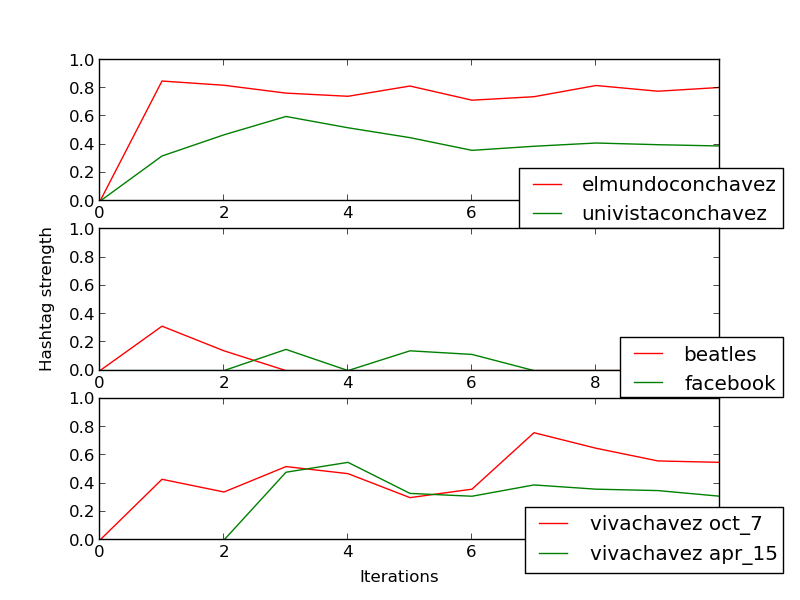
\includegraphics[scale=0.40]{support_files/hashTagTimeSeries.png}\\
	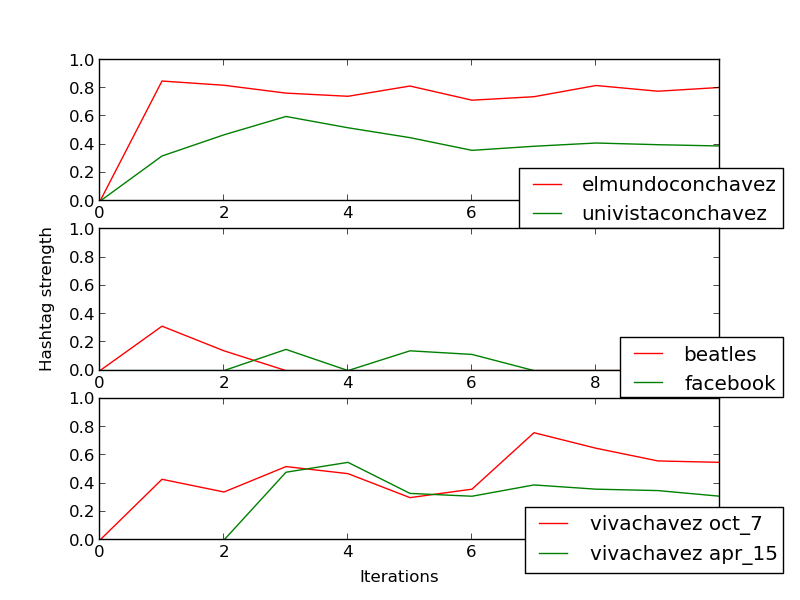
\includegraphics[height=0.2\textheight, width=0.45\textwidth]{support_files/hashTagTimeSeries.png}
	\caption{Time series comparison for different hashtags identified for Hugo Ch\'{a}vez.}
	\label{fig:timeSeries}
\end{figure}
In Figure~\ref{fig:timeSeries}, the first plot elucidates how hashtags like \emph{``elmnduconchavez"} and 
\emph{``univistaconchavez"} remain highly associated with Hugo Ch\'{a}vez for the October 7th Presidential election. 
These hashtags remain indicative of a user's affiliation throughout the month leading up to the election.
Meanwhile hashtags such as \emph{"beatles"} and \emph{"facebook"} (in second plot) show spikes in their time series primarily because users affiliated with Ch\'{a}vez used them during that time window. 
But as the iterative process continues, the system drops these non-informative words.
The third plot presents another interesting observation.
Hugo Ch\'{a}vez who had won the election on October 7, 2012 was diagnosed with cancer and passed away
before being sworn in as the President.
This triggered a re-election on April 15, 2013 where Nicolas Maduro, who had assumed the role of acting president then, competed 
against Henrique Capriles in the Presidential race.
The hashtag \emph{``vivachavez"} is part of both the elections, despite the 
fact that Hugo Ch\'{a}vez did not compete in the second election.
It is picked up as a phrase commonly used by supporters of Nicholas Maduro whose election campaign was strategized around the death of Hugo Ch\'{a}vez to garner sympathy and mobilize support.
Similarly variations of the hashtags \emph{``hayuncamino"} and \emph{``unidadvenuzela"} were returned 
for Henrique Capriles for both these elections.
The tag MUD is for ``Mesa de la Unidad Democratica” (Democratic Unity Roundtable) that was the organization created for the opposition to Ch\'{a}vez. 
The vocabulary grows to include other terms associated to the campaign, as the official slogan for the opposition ``hayuncamino” (there is a road). 
Others relate to programs that Capriles wanted to implement, such as ``planprimerempleo” (First Job Program). 

\noindent	
{\bf Mexico:} A general election in Mexico took place on July 1st, 2012.
The two front runners where Enrique Pe\'{n}a Nieto (EPN) and Andres Manuel L\'{o}pez Obrador (AMLO).
The tags (Figure~\ref{fig:mexicowordCloud}) show the contest between these two candidates, the first belonging to the “Partido Institucional Revolucionario” (PRI). 
Among the tags we can also find reference to the “yosoy132” student movement that became a key player during the election. 
%We have against AMLO some as “niunvotoalpeje” (no one vote for AMLO) or against EPN “soyantipri” (I am against PRI).
We also see “niunvotoalpeje” (no one vote for AMLO) and “soyantipri” (I am against PRI) which are attributed against AMLO and EPN respectively.

\noindent
{\bf Paraguay:}
Figure~\ref{fig:paraguaywordCloud} details the election between Horacio Cartes from the Partido Colorado and Efrain Alegre from Alianza Paraguay. 
The incumbent president belonged to Partido Colorado and we can see some tags talking about a protest vote: “votocastigoya” (protest vote now). 
Also references from their campaign to each candidate as “yovotoporefrain” (I vote for efrain) or “todosconcartesavanzapais” (everyone with cartes, the country goes forward) are seen.

\noindent
{\bf Honduras:}
In November 2013 Honduras had a general election to choose President, Congress and local officials. 
The wife of former President Zelaya, Xiomara Castro, contended against Juan Orlando Hernandez from the incumbent Partido Nacional. 
Both candidates showed similar numbers in the polls before the election. 
We can find tags that either support Xiomara, like “xiomarapresidenta” (Xiomara President), “hondurastienepresidenta” (Honduras has a female president) or against her, “noaxiomara” (no to Xiomara) in Figure~\ref{fig:honduraswordCloud}.

\noindent
{\bf Ecuador:}
Ecuador had a first round for the presidential election on February 17th, 2013 where Rafael Correa obtained more than 50\% of the votes needed to avoid a second round. 
From the tags(Figure~\ref{fig:ecuadorwordCloud}) we can read support in phrases such as “yatenemospresidente” (we have elected president) or “tenemosarafael” (we have Rafael). 
There are some references to other candidates such as “lassopresidente” (candidate Lasso president).

\noindent
{\bf Colombia:}
The hashtags identified for Juan Manuel Santos who won the Colombian Presidential elections in the second round,
June 15(first round May 25). The query expansion pipeline for these elections were initialized only with the main two candidates names: Santos, Manuel and Zuluaga, Ivan.

\noindent
{\bf Panama:}
Panama's presidential election was held on May 4, with Juan Carlos Varela the winner. Seeding the query expansion pipeline were the last names of the candidates(Arias, Varela and Navarro) plus the initials of their parties(CD, PP and PRD respectively), with the addition of Arias' first name 'Domingo' to distinguish him from a former president, Oscar Arias.

\begin{figure}
	\centering
	\subfloat[Nov 24]
	{
		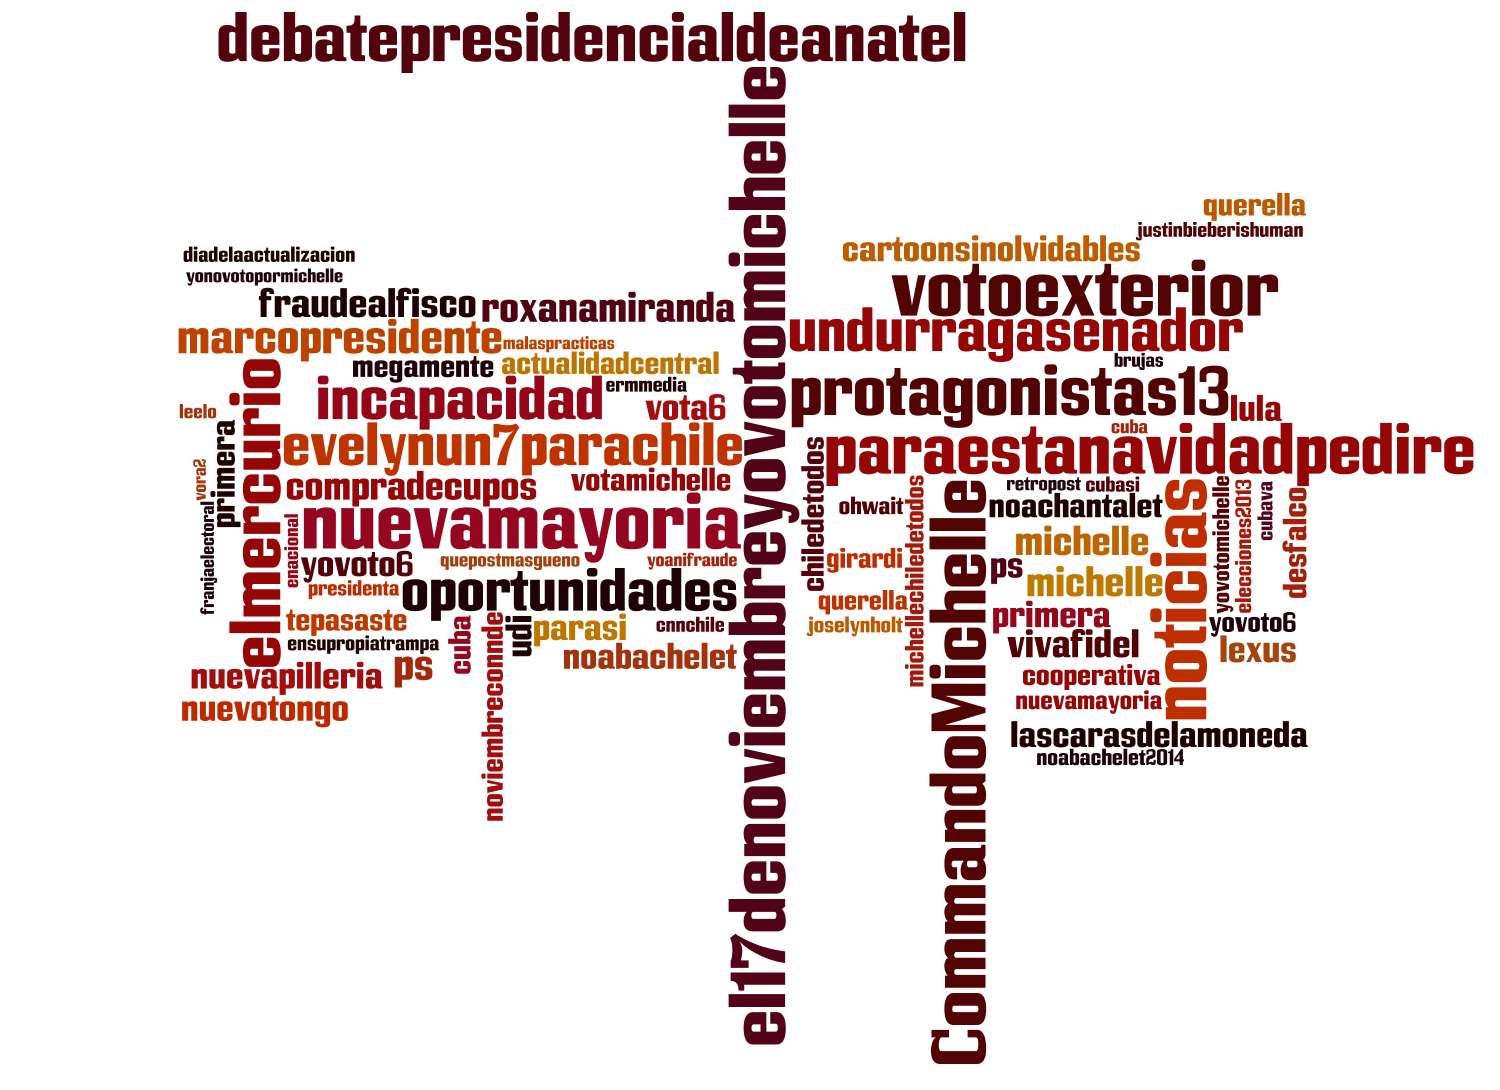
\includegraphics[width=0.22\textwidth, height=0.15\textheight]{support_files/bacheletWordCloud1.png}
		\label{fig:bacheletwordCloud1}
	} 
	\subfloat[Dec 15]
	{
		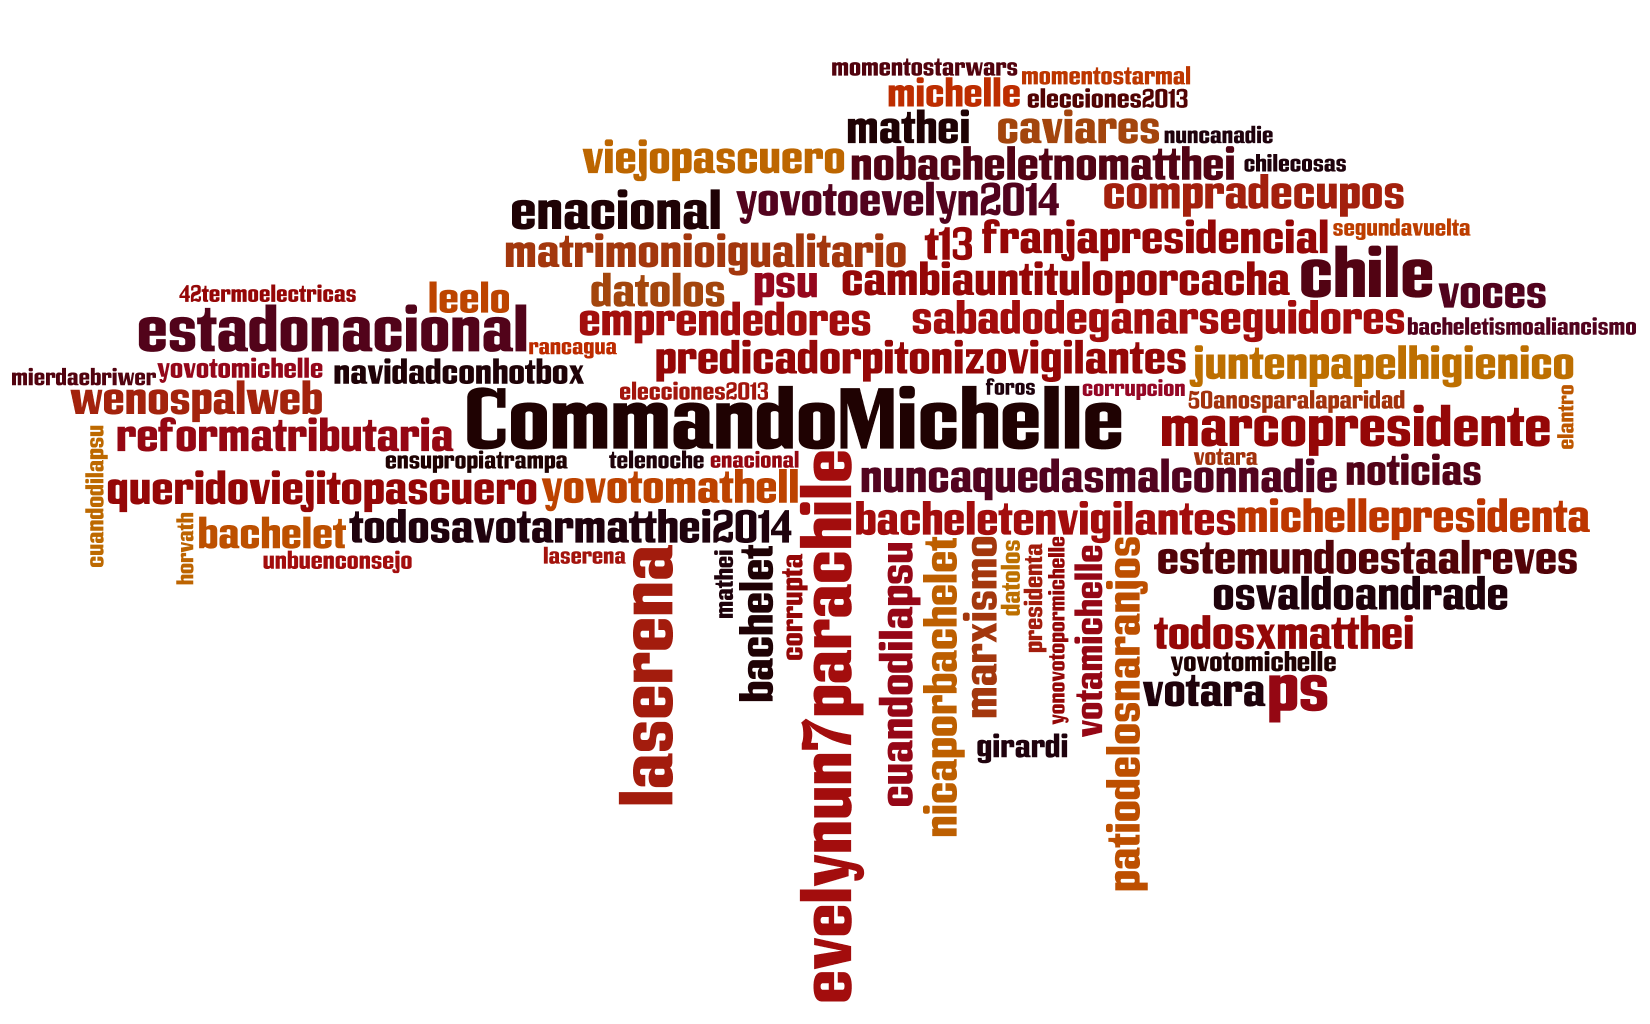
\includegraphics[width=0.22\textwidth, height=0.15\textheight]{support_files/bacheletWordCloud2.png}
		\label{fig:bacheletwordCloud2}
	}
	\caption{Hashtags identified for Michelle Bachelet} 
	\label{fig:bacheletwordCloud}
\end{figure}

{\bf Chile:}
Figure~\ref{fig:bacheletwordCloud} shows the hashtags identified for Michelle Bachelet who won the Chilean Presidential elections that was decided over two rounds.
The first round was conducted on the 24th of November, 2013 and the 2nd round was conducted on December 15, 2013. 
The query expansion pipeline for Bachelet's group in both these elections were initialized only with three seed words: {\it Bachelet, CommandoMichelle and PS}. 
The first name of the candidate was not used as it introduced a lot of noise because ``Michelle" is a very common name.
The first figure shows the hashtags identified for Bachelet during the first round and the second figure for the second round. 
It can be seen that there is a lot of overlap in the vocabulary which is the expected outcome. 
Similarly there were a lot of common hashtags between the two rounds of election for the other candidate, Evelyn Matthei, too.
%Figure~\ref{fig:countrywordCloud} shows the hashtags identified for the elections from Mexico, Paraguay, Honduras and Ecuador. 
It can be noticed that the vocabulary for the Honduran and Ecuadorean  elections are quite noisy. 
This is primarily because Twitter is not as popular in these two countries as in Venezuela or Chile and therefore the number of tweets
used for the inference was significantly lesser.
This in turn affects the quality of the PSL inference.


\begin{figure}[t]
	\centering
	\subfloat[Mexico]
	{
		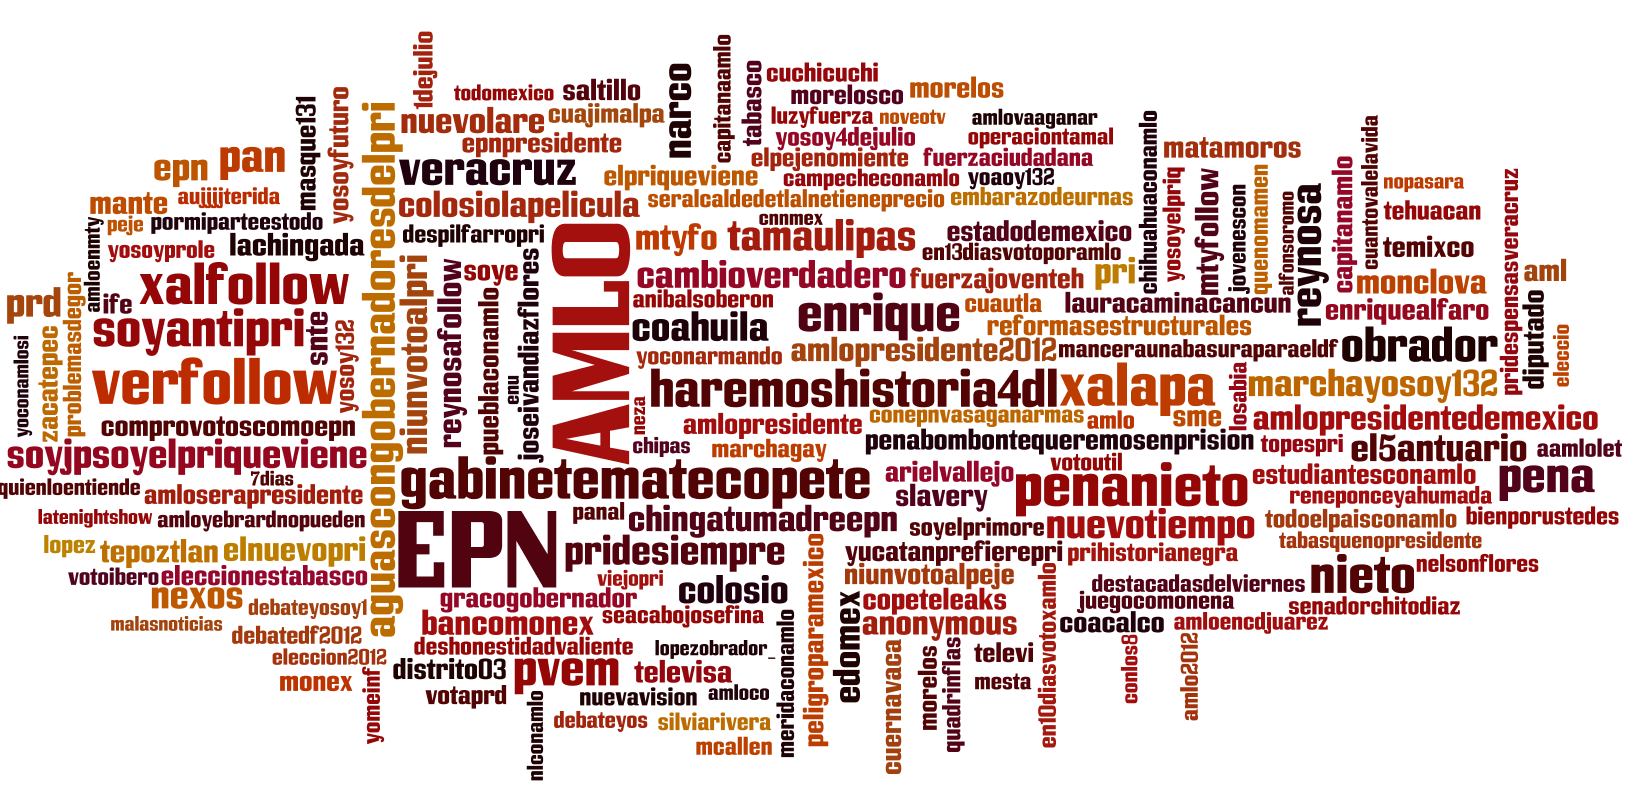
\includegraphics[width=0.22\textwidth, height=0.15\textheight]{support_files/mexicoWordCloud.png}
		\label{fig:mexicowordCloud}
	} 
	\subfloat[Paraguay]
	{
		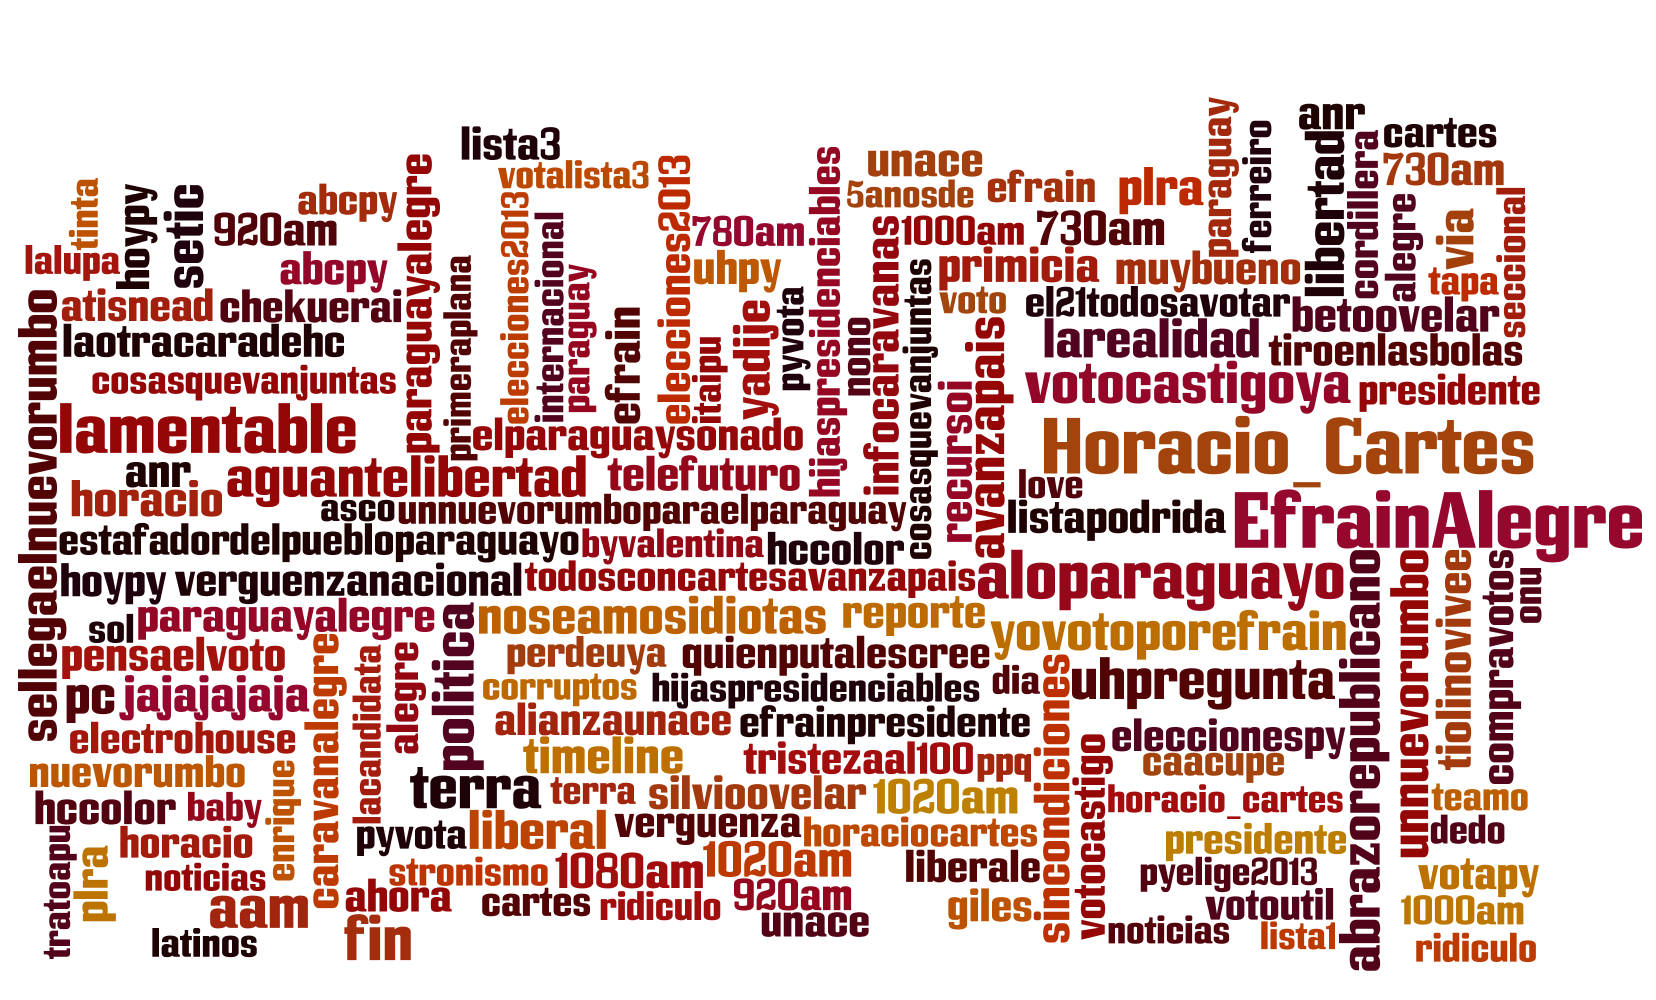
\includegraphics[width=0.22\textwidth, height=0.15\textheight]{support_files/paraguayWordCloud.png}
		\label{fig:paraguaywordCloud}
	} \\
	\noindent 
	\subfloat[Honduras]
	{
		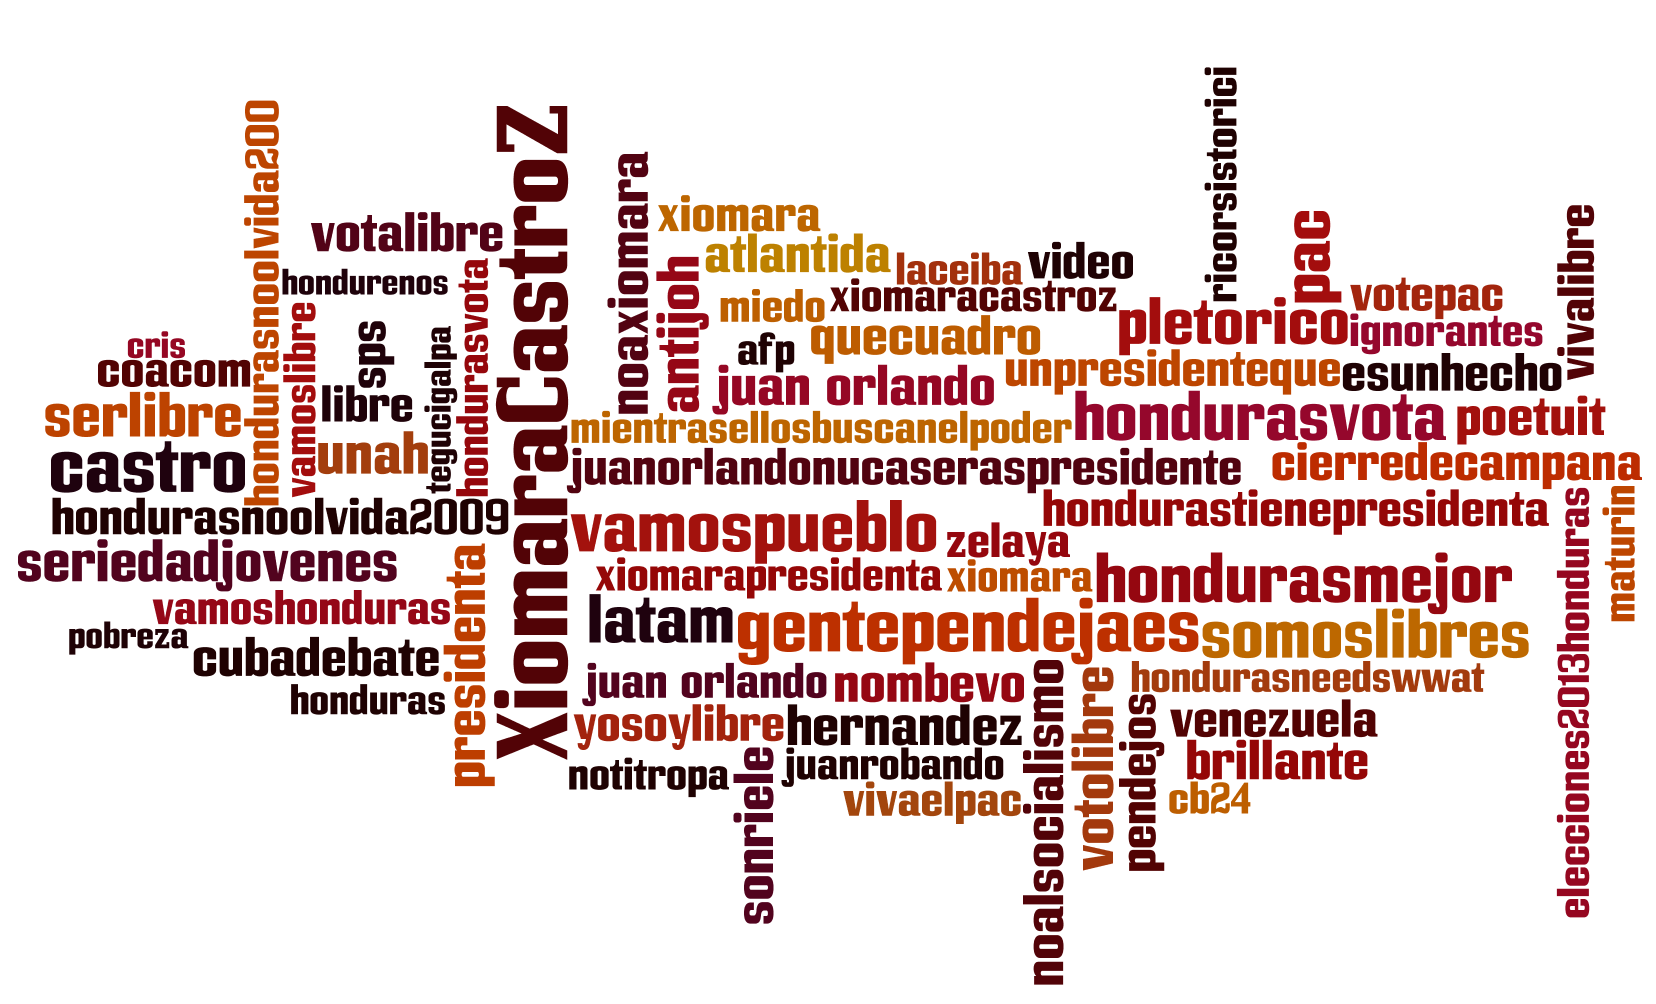
\includegraphics[width=0.22\textwidth, height=0.15\textheight]{support_files/hondurasWordCloud.png}
		\label{fig:honduraswordCloud}
	}
	\subfloat[Ecuador]
	{
		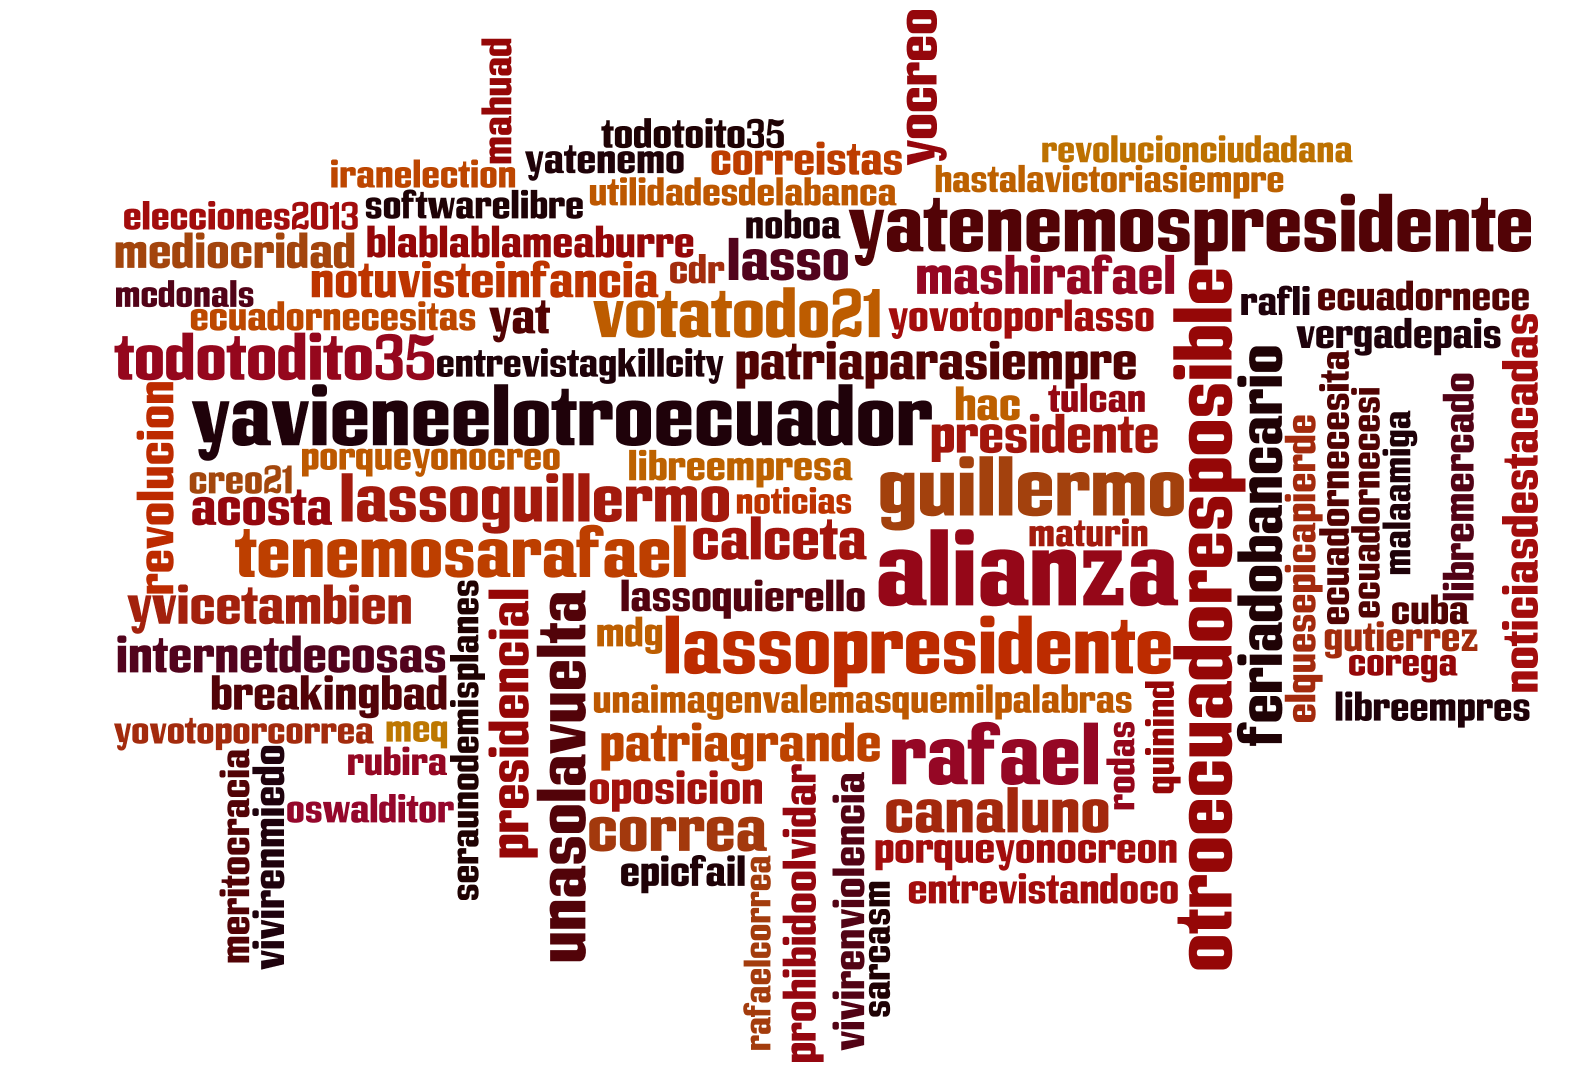
\includegraphics[width=0.22\textwidth, height=0.15\textheight]{support_files/ecuadorWordCloud.png}
		\label{fig:ecuadorwordCloud}
	}\\
	\noindent 
	\subfloat[colombia]
	{
		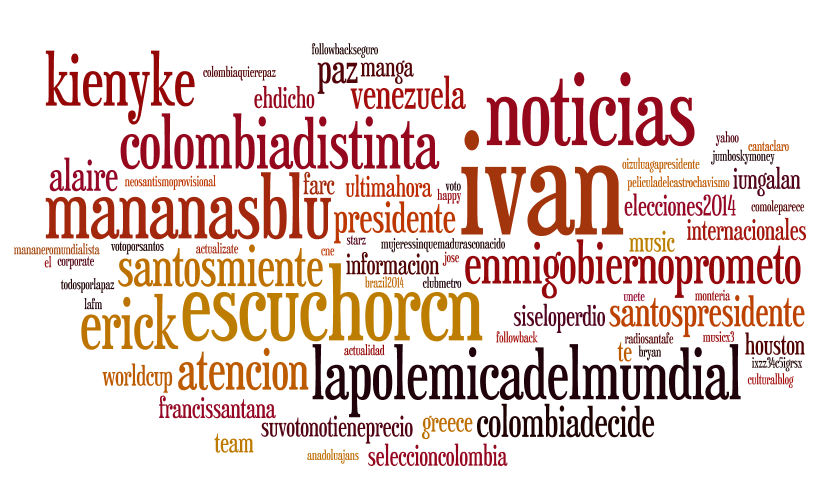
\includegraphics[width=0.22\textwidth, height=0.15\textheight]{support_files/colombia_cloud.png}
		\label{fig:colombiawordCloud}
	}
	\subfloat[panama]
	{
		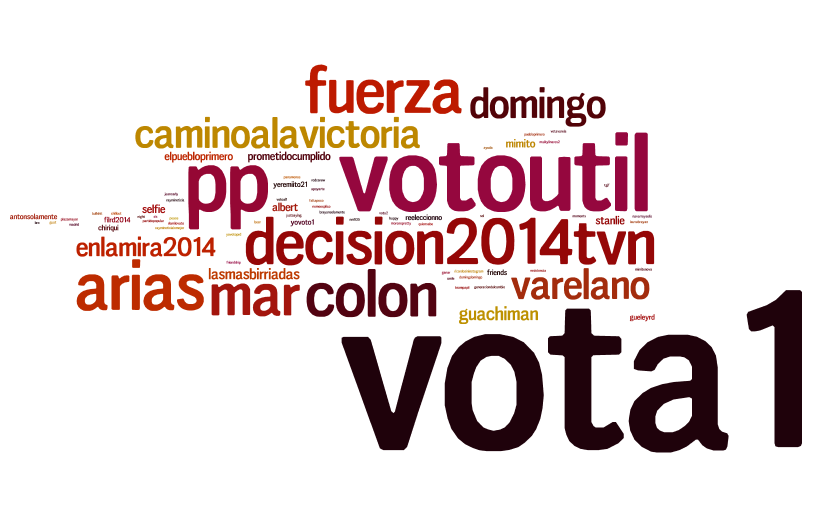
\includegraphics[width=0.22\textwidth, height=0.15\textheight]{support_files/panama_cloud.png}
		\label{fig:panamawordCloud}
	}
	\caption{Vocabulary of hashtags identified for different elections} 
	\label{fig:countrywordCloud}
\end{figure}
\noindent

